\chapter{Implementasi dan Pengujian Perangkat Lunak}
\label{chap: Implementasi dan Pengujian Perangkat Lunak}

Bab ini terdiri atas tiga bagian, yaitu Implementasi Data JSON, Implementasi Perangkat Lunak dan Pengujian Perangkat Lunak. Bagian implementasi data json akan berisi di mana json akan disimpan, lalu implementasi perangkat lunak berisi penjelasan lingkungan pengembangan perangkat lunak. Sedangkan bagian pengujian berisi hasil pengujian fungsional terhadap perangkat lunak yang telah dibangun dan pengujian eksperimental yang isinya percobaan pada setiap \textit{engine} yang digunakan dalam pembuatan pohon kurikulum.

\section{implementasi data json}
\label{sec: implementasi data json}

Dalam pembangunan pohon kurikulum digunakan JSON sebagai data yang akan di olah. JSON dibangkitkan dengan cara di ubah menjadi menjadi \textit{dot}. Setelah di ubah maka dapat dilihat hasilnya berupa grafik yang berbentuk pohon kurikulum. JSON selanjutnya di unggah dan diakses melalui \textit{url} \url{https://github.com/ftisunpar/data} dan dilihat pada bagian prasyarat. Hasil implementasi pada pohon kurikulum isinya bergantung pada hasil implementasi JSON yang di unggah pada \textit{url} tempat JSON disimpan.

\section{Implementasi Perangkat Lunak}
\label{sec: Implementasi Perangkat Lunak}

Pada bagian ini akan dibahas mengenai implementasi perangkat lunak yang telah dibangun. Sub bab ini terdiri atas tiga bagian, yaitu lingkungan perangkat lunak, hasil implementasi perangkat lunak, dan Pengujian fungsional.

\subsection{Lingkungan Implementasi Perangkat Lunak}
\label{sec: Lingkungan Implementasi Perangkat Lunak}

Dalam proses membangun perangkat lunak ini digunakan spesifikasi perangkat sebagai berikut:

\begin{enumerate}
\item Lingkungan Pembangunan 
\begin{itemize}
\item Processor : Intel Corei7-4702MQ 2.2-3.2GHz
\item RAM : 4.00 GB
\item Harddisk : 1TB
\item VGA : NVIDIA GeForce GT 740M
\item Sistem Operasi Komputer : Windows 10 Education 64-bit
\end{itemize}

\item Lingkungan Implementasi
\begin{itemize}
\item Tools : \textit{Visual Studio Code}
\item Bahasa Pemrograman : Javascript
\item Framework : \textit{viz.js}
\end{itemize}

\end{enumerate}

\subsection{Hasil Implementasi}
\label{sec: Hasil Implementasi}

Kode program pada perangkat lunak ditulis dalam bahasa pemrograman \textit{javascript} dengan cara membangkitkan dari JSON ke \textit{DOT}. Hasil implementasi berupa pohon kurikulum yang visualisasinya menggunakan \textit{viz.js}. Perangkat lunak dapat dilihat seperti gambar di bawah ini.

\begin{figure}[H]
		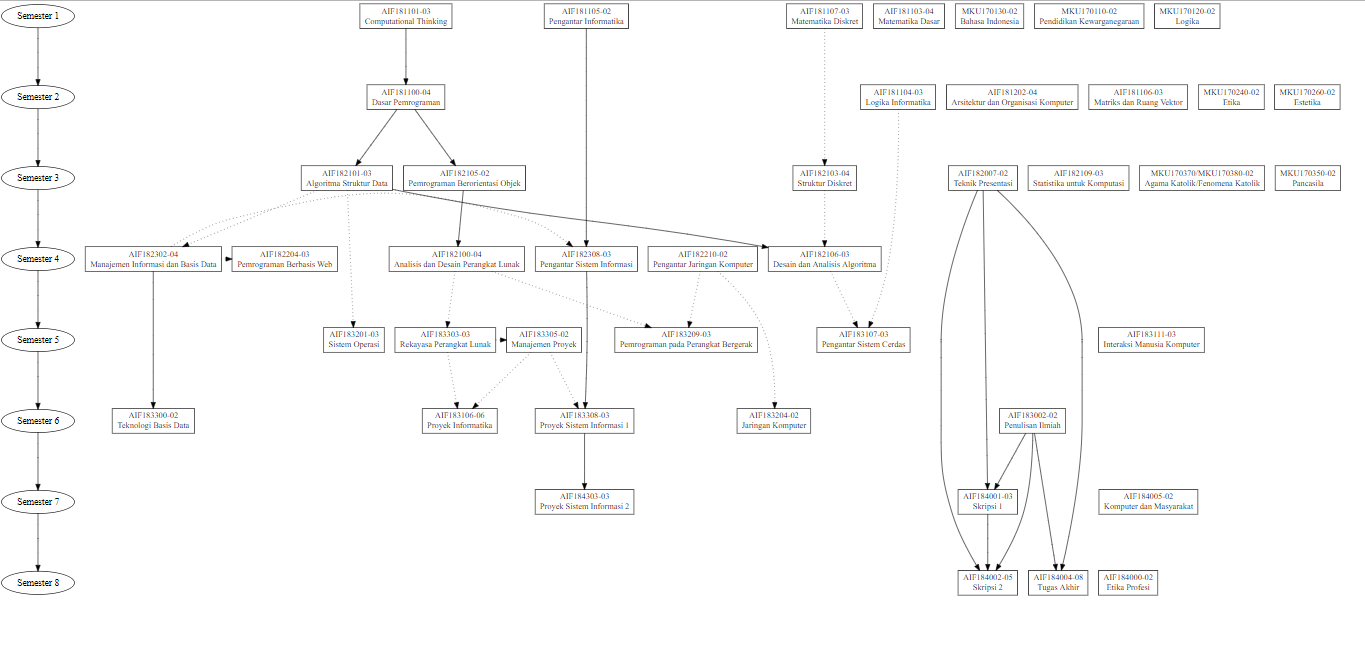
\includegraphics[scale = 0.5]{pohonkurikulum.png}
		\caption{Hasil Implementasi}
		\label{fig: pohon kurikulum}
\end{figure}	 

Pada gambar \ref{fig: pohon kurikulum} terlihat setiap semester memiliki mata kuliah yang berisi semester, kode mata kuliah, jumlah sks, dan nama mata kuliah. Lalu mata kuliah yang memiliki prasyarat akan ditunjuk oleh panah. Syarat yang menjadi patokan adalah syarat tempuh, syarat lulus, atau pengambilan secara bersamaan.

\section{Pengujian Perangkat Lunak}
\label{sec: Pengujian Perangkat Lunak}

Pada bab ini akan dibahas mengenai pengujian perangkat lunak yang dibangun. Pengujian yang dilakukan adalah pengujian fungsional dan pengujian eksperimental. Pengujian fungsional bertujuan untuk memastikan bahwa seluruh fungsi perangkat lunak yang dibangun berjalan sesuai dengan rencana dan pengujian eksperimental bertujuan untuk mengetahui apa saja \textit{engine} yang dapat dipakai dalam membangun perangkat lunak.

\subsection{Pengujian Fungsional}
\label{sec: Pengujian Fungsional}
Dalam sub bab ini akan dilakukan pengujian fungsional untuk mengetahui fungsi-fungsi yang terdapat
pada perangkat lunak dapat berjalan sesuai dengan yang diharapkan. Status pengujian dibagi
menjadi dua yaitu "ok" dan "gagal". Di bawah ini Pengujian fungsi pohon kurikulum:

\begin{table}[H]
\begin{center}
\caption{Hasil Pengujian Fungsional}
\begin{tabular}{{|p{2cm}|p{3cm}|p{4cm}|p{1cm}|}}
\hline
  Pengujian & Tujuan Pengujian & Hasil Pengujian & Status \\
\hline
  Memanggil fungsi rankSep & Mengeluarkan node semester dan kode mata kuliah wajib & node semester satu sampai delapan dan kode mata kuliah berhasil diketahui & ok\\ \hline
	Memanggil fungsi nodesMatkul & fungsi nodesMatkul akan mengeluarkan label yang berisi kode, sks, dan nama mata kuliah & kode, sks, dan nama mata kuliah wajib berhasil ditampilkan & ok\\ \hline
	Memanggil fungsi edgesMatkul & Mata kuliah yang mempunyai prasyarat bisa diketahui melalui petunjuk arah & Mata kuliah yang memiliki prasyarat akan ditunjuk sesuai prasyarat. Jika syaratnya lulus maka garis akan lurus jika syaratnya tempuh garis putus-putus & ok\\ \hline
   
\end{tabular}
\end{center}
\end{table}

\subsection{Pengujian Eksperimental}
\label{sec: Pengujian Eksperimental}

Pengujian eksperimental dilakukan dengan cara membuat beberapa tugas dalam pembuatan pohon kurikulum. Tujuan yang ingin dicapai dalam pengujian eksperimental ini untuk memastikan seluruh \textit{engine} dapat digunakan perangkat lunak dengan mudah dan sesuai harapan. Metode pengumpulan data dalam pengujian eksperimental ini adalah hasil dari pengujian setiap \textit{engine}. Mengacu pada bab 2 bagian Visualisasi Graf dengan \textit{viz.js} di sana disebutkan \textit{engine} yang dapat digunakan untuk menampilkan grafik.

\begin{enumerate}
\item \textit{Engine= dot}, akan menghasilkan sebuah grafik seperti gambar di bawah ini.
\begin{figure}[H]
		\left
		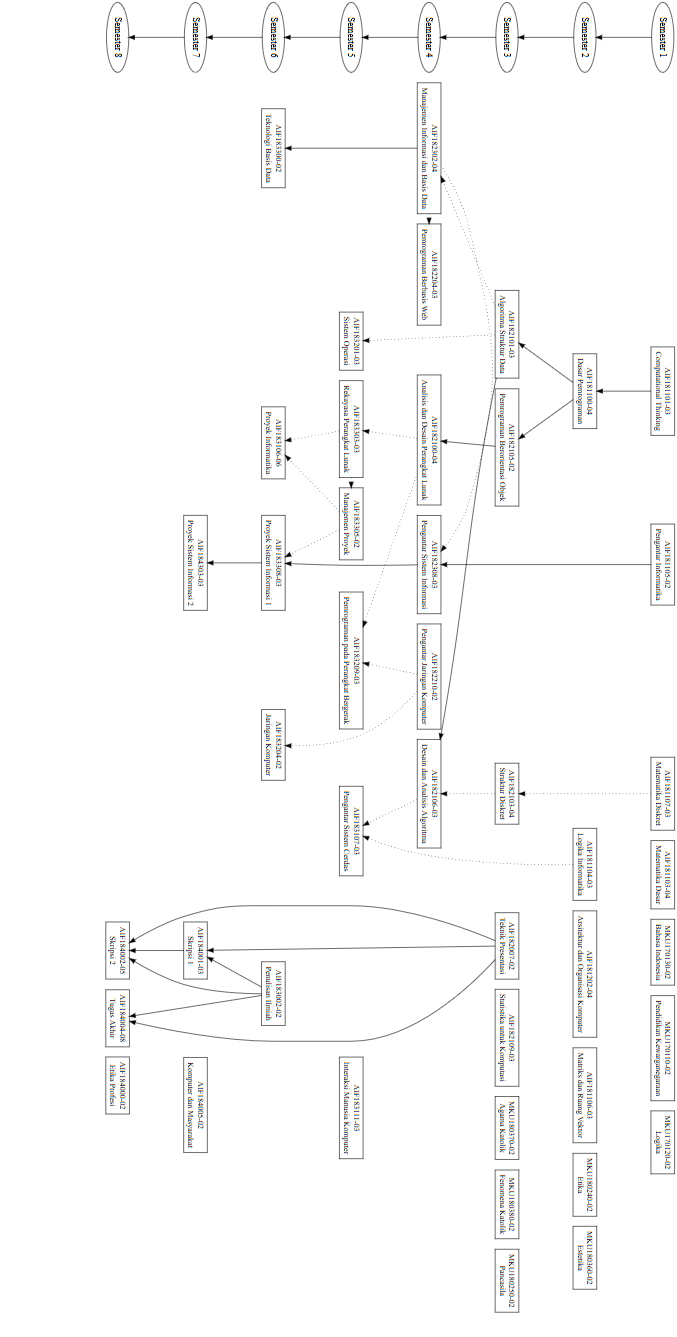
\includegraphics[scale = 0.5]{dot.png}
		\caption{Hasil dot}
		\label{fig: dot}
\end{figure}

\item \textit{Engine= circo}, akan menghasilkan sebuah grafik seperti gambar di bawah ini.
\begin{figure}[H]
		\left
		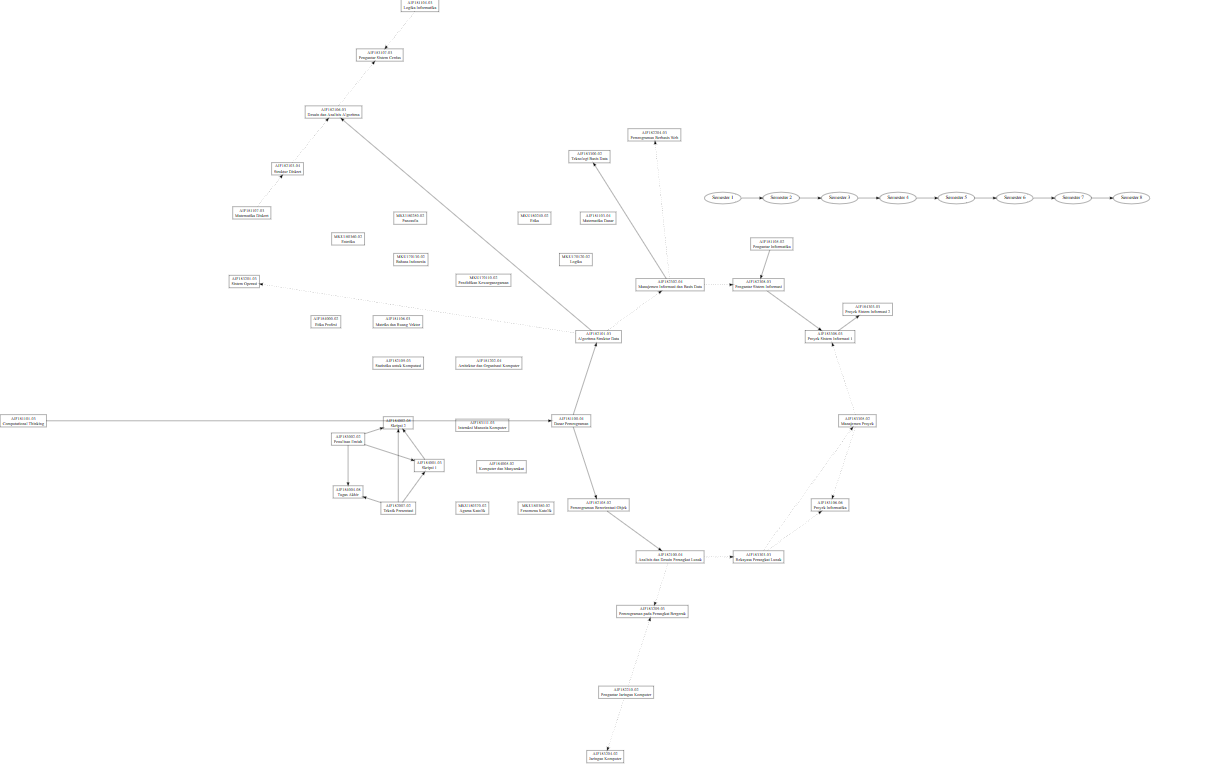
\includegraphics[scale = 0.5]{circo.png}
		\caption{Hasil circo}
		\label{fig: circo}
\end{figure} 

\item \textit{Engine= fdp}, akan menghasilkan sebuah grafik seperti gambar di bawah ini.
\begin{figure}[H]
		\left
		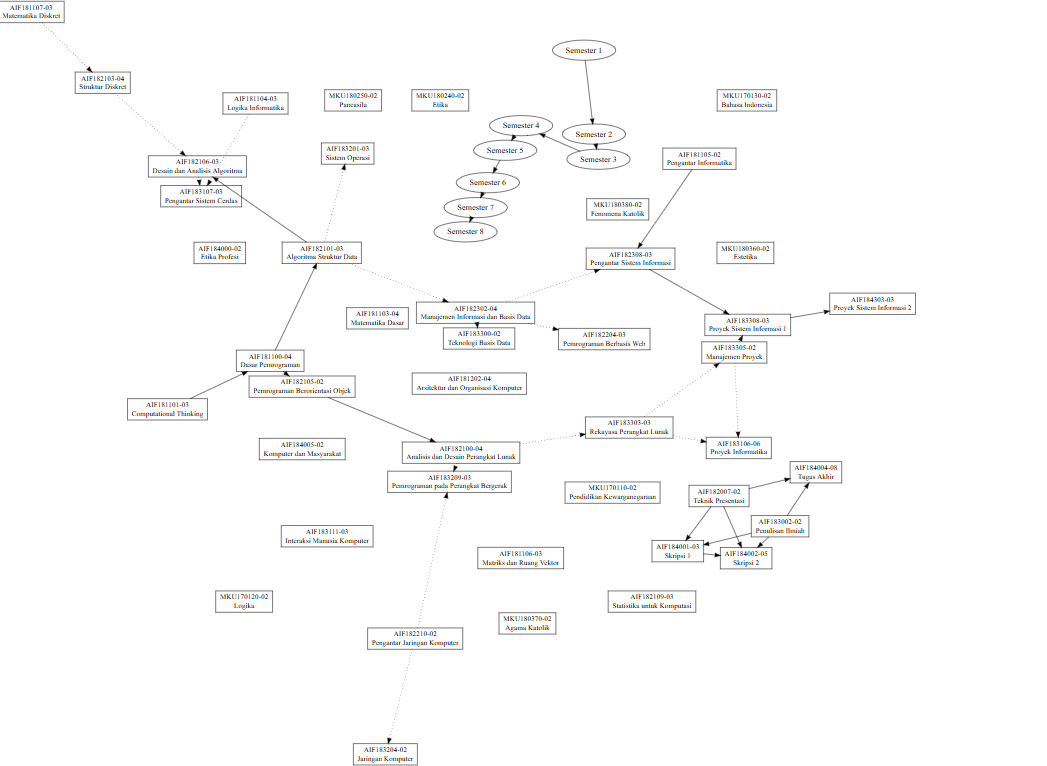
\includegraphics[scale = 0.5]{fdp.png}
		\caption{Hasil fdp}
		\label{fig: fdp}
\end{figure}

\item \textit{Engine= neato}, akan menghasilkan sebuah grafik seperti gambar di bawah ini.
\begin{figure}[H]
		\left
		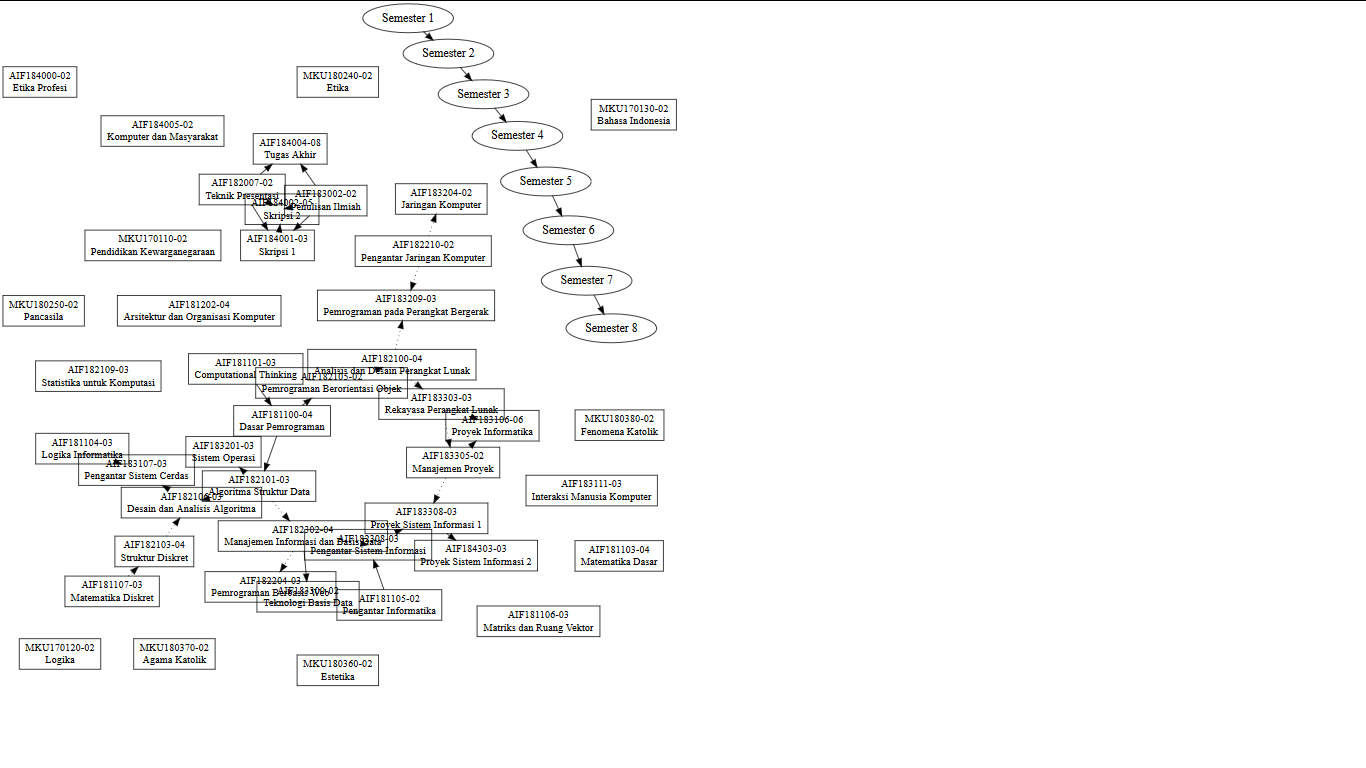
\includegraphics[scale = 0.5]{neato.png}
		\caption{Hasil neato}
		\label{fig: neato}
\end{figure}

\item \textit{Engine= osage}, akan menghasilkan sebuah grafik seperti gambar di bawah ini.
\begin{figure}[H]
		\left
		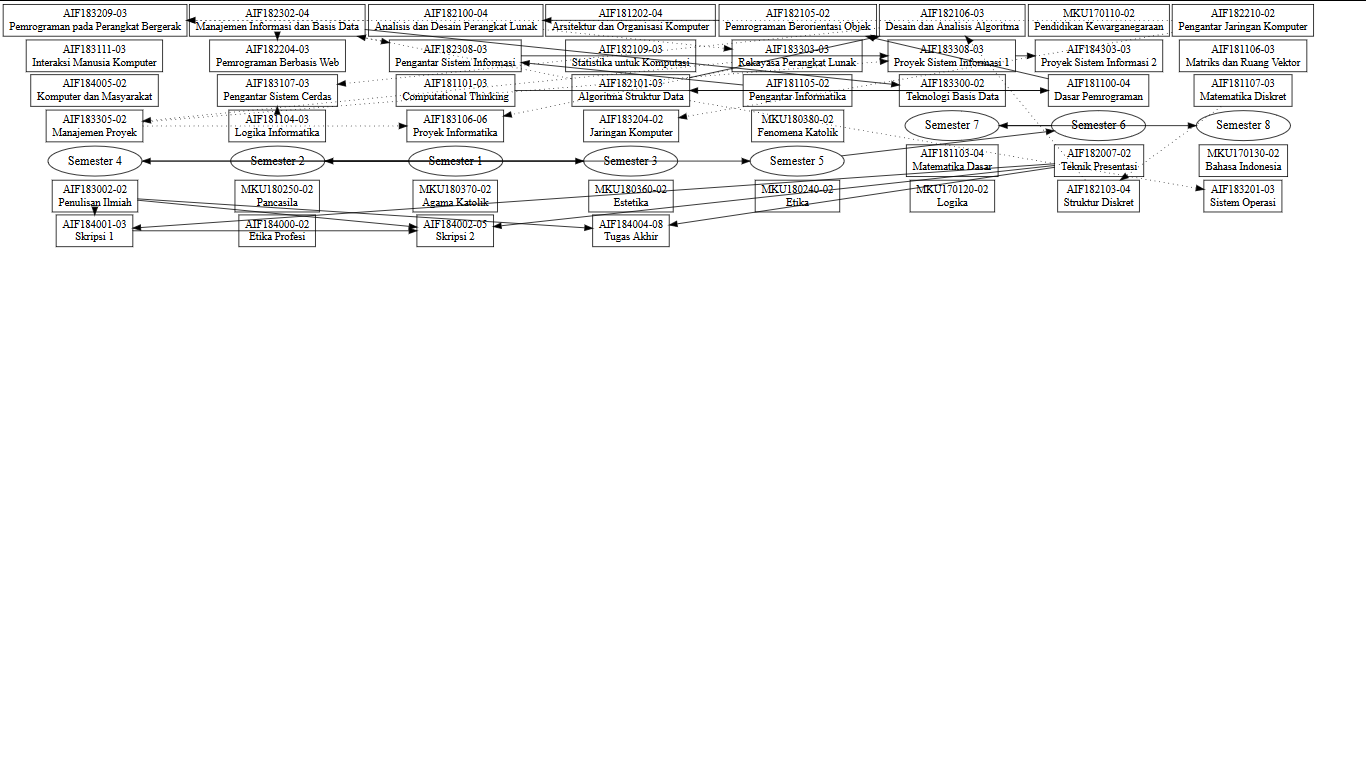
\includegraphics[scale = 0.5]{osage.png}
		\caption{Hasil osage}
		\label{fig: osage}
\end{figure}

\item \textit{Engine= twopi}, akan menghasilkan sebuah grafik seperti gambar di bawah ini.
\begin{figure}[H]
		\left
		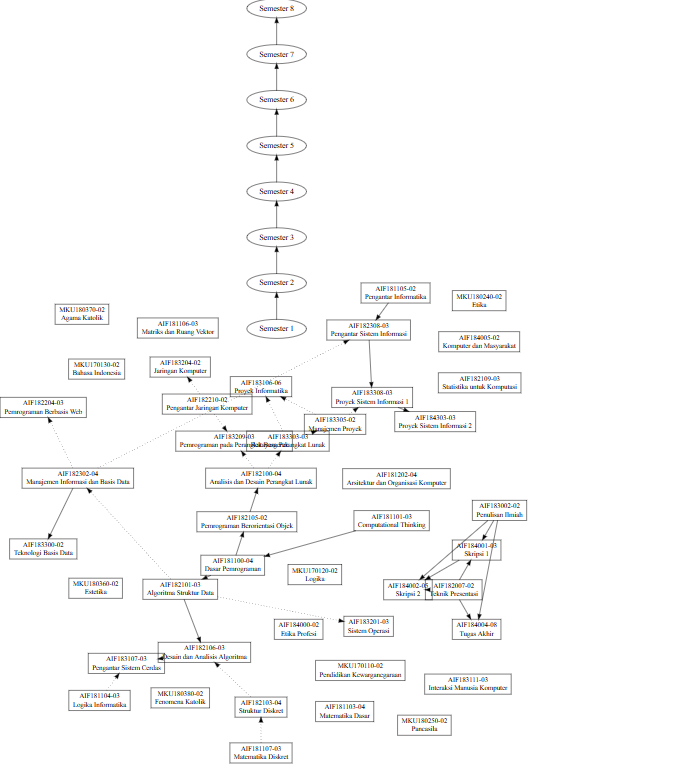
\includegraphics[scale = 0.5]{twopi.png}
		\caption{Hasil twopi}
		\label{fig: twopi}
\end{figure}

\end{enumerate}